\chapter{Fire prevention}
	\section{Fire prevention regulations }
	For fire prevention, ANNEX 14 V1 from ICAO, \cite{Standards2016} and Airport Service Manual regulations will be taken into account, \cite{InternationalCivilAviationOrganisation2014}.
		\subsection{Level of protection}
		\paragraph{} From ICAO Annex 14 V1, \cite{Standards2016}, the level of protection at an aerodrome for rescue and firefighting should be equal to aerodrome category determined using the principles in articles \textit{9.2.5} and \textit{9.2.6}.
		
		Table \ref{table91} is used to determine the aerodrome category taking into account the longest aeroplanes normally using the aerodrome.
		
		The biggest plane using the aerodrome is the Boeing 777-300 which have a length of 74m and a fuselage width of 6.2m.
		
		According to this data, the \textbf{Aerodrome category} is \textbf{9}.
		
		\begin{figure}[H]
			\centering
			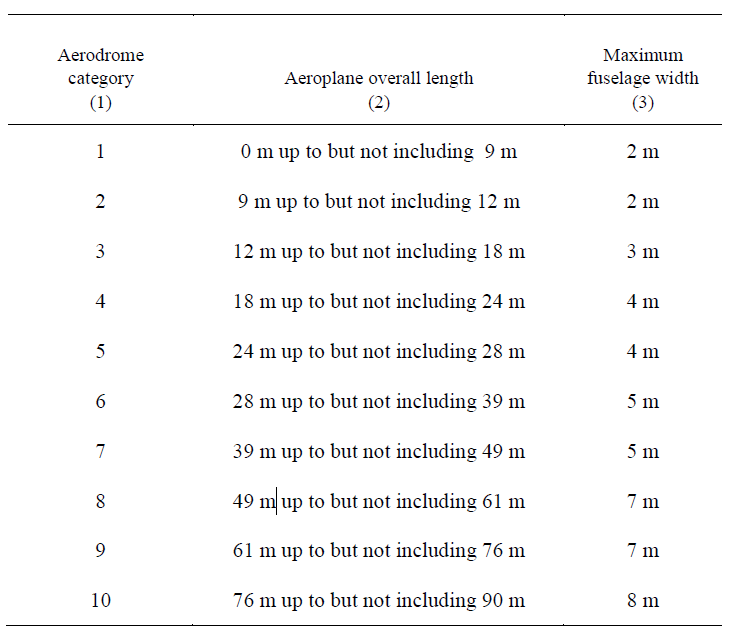
\includegraphics[clip, trim=0cm 0cm 0cm 0cm, width=0.8\textwidth]{./images/firefighting/table91}
			\caption{Aerodrome category for rescue and firefighting.}
			\label{table91}
		\end{figure}
	
		\subsection{Extinguishing agents}
		\paragraph{} Also, from ICAO Annex 14 V1, \cite{Standards2016}, section 9, the amounts of water for foam production and the complementary agents to be provided on the rescue and firefighting vehicles shall be in accordance with the aerodrome category.
		
		From \textit{Airport Services Manual (Doc 9137), Part 1}, \cite{InternationalCivilAviationOrganisation2014} and the category of the airport, the level of performance selected is \textbf{level A}. Now the table \ref{table92} can be used to determine the minimum usable amount of extinguishing agents for the airport.  
		\begin{figure}[H]
			\centering
			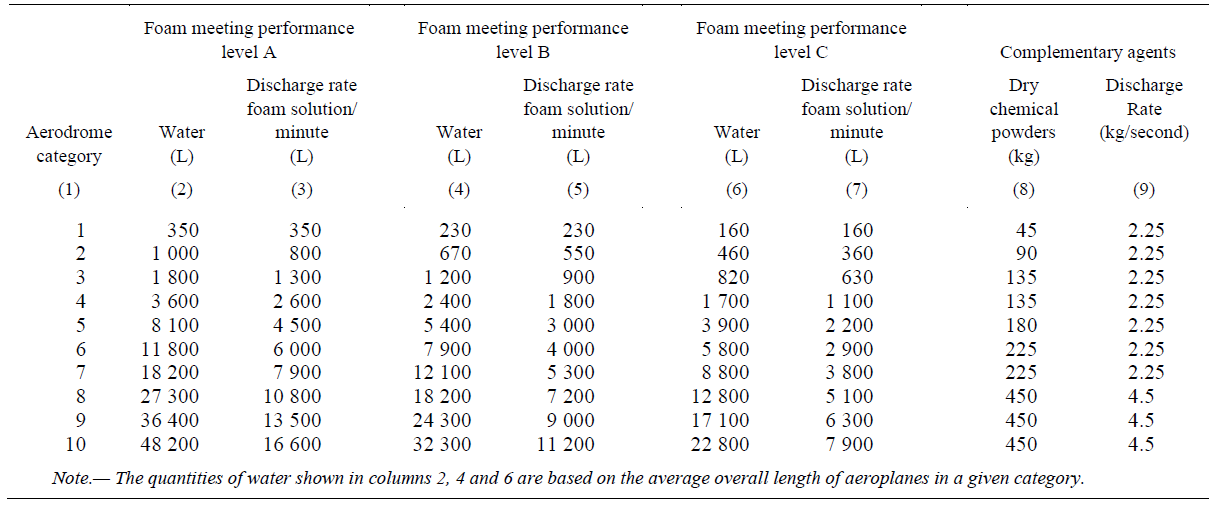
\includegraphics[clip, trim=0cm 0cm 0cm 0cm, width=1\textwidth]{./images/firefighting/table92}
			\caption{Minimum usable amount of extinguishing agents.}
			\label{table92}
		\end{figure}
	
	For a category 9 aerodrome with performance level A, the minimum usable amount of water is 36400 L and 13500 discharge rate foam solution per minute, for 450kg of dry chemical powders with a discharge rate of 4.5kg/s.

	Following the directives from article 9, the amount of foam concentrate provided on a vehicle should be sufficient to produce at least two loads of foam solution. Foam concentrate carried on fire vehicles in excess of the quantity identified in Table \ref{table92} can contribute to the reserve.
	
		\subsection{Rescue equipment}
Rescue equipment commensurate with the level of aircraft operations should be provided on the rescue and firefighting vehicle(s).
		\subsection{Response time}
		The operational objective of the rescue and firefighting service shall be to achieve a response time not exceeding three minutes to any point of each operational runway, in optimum visibility and surface conditions.
		
		On the figure \ref{schemeFire}, the firefighting station location over the airport can be seen along the distances to the runways headers.
		
		Considering a conservative value for the average velocity of a fire truck, around 60km/h. Is possible to state that the response time doesn't exceed the three minutes to any point of each operational runway. The response time for a the farthest runway header (01R) is 2min 40s, giving a 20s margin for fire-fighters to put its equipment on. 
		\begin{figure}[H]
			\centering
			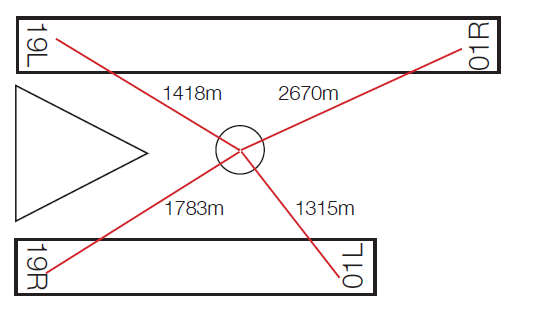
\includegraphics[clip, trim=0cm 0cm 0cm 0cm, width=0.8\textwidth]{./images/firefighting/schemeFire}
			\caption{Firefighting station location with runways headers distances.}
			\label{schemeFire}
		\end{figure}
		
		Any vehicles, other than the first responding vehicle(s), required to deliver the amounts of extinguishing agents specified in Table \ref{table92} shall ensure continuous agent application and shall arrive no more than four minutes from the initial call.
		
		Additionally Jakarta Fire-fighters station is at 25 km away and could provide auxiliary support.
		
		\subsection{Emergency access roads}
		\paragraph{} Tanks to the airport is on a perfectly flat terrain, is possible to go across the concrete terrain, following an straight line to the headers. There are also, auxiliary roads near to the taxiways.
		
		\subsection{Fire stations}
		Fire-Fighters station with two floors linked with vertical slide bars and stairs. 
		
		\begin{description}
			\item[Ground level:] a quick and direct garage for 3 vehicles, plus lockers and depot.
			\item[First floor] with all the facilities such as gym, rest area, bedrooms, washroom, dinning room and infirmary.
		\end{description}
			
	\subsection{Number of rescue and firefighting vehicles}
	According to Table \ref{table9241}, the minimum number of rescue and firefighting vehicles provided at an aerodrome should be 3, because aerodrome is category 9.
	\begin{figure}[H]
		\centering
		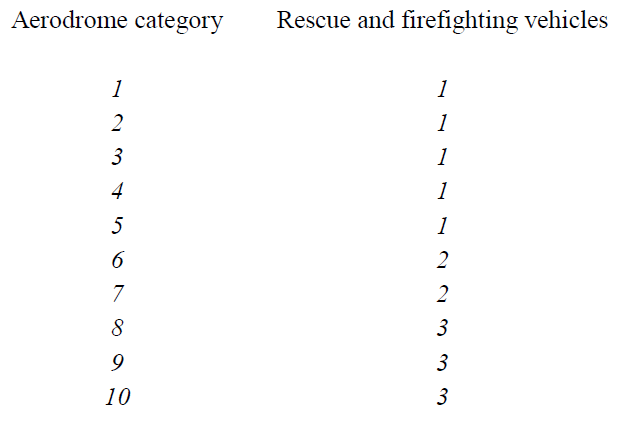
\includegraphics[clip, trim=0cm 0cm 0cm 0cm, width=.6\textwidth]{./images/firefighting/table9241}
		\caption{Minimum characteristics of rescue and firefighting vehicles.}
		\label{table9241}
	\end{figure}
	\subsection{Personnel}
	\paragraph{} All rescue and firefighting personnel shall be properly trained to perform their duties in an efficient manner and shall participate in live fire drills commensurate with the types of aircraft and type of rescue and firefighting equipment in use at the aerodrome, including pressure-fed fuel fires.
	
	The rescue and firefighting personnel training programme shall include training in human performance, including team coordination.
	
	All responding rescue and firefighting personnel shall be provided with protective clothing and respiratory equipment to enable them to perform their duties in an effective manner.
	
	Sufficient trained and competent personnel will be designated to be readily available to ride the rescue and firefighting vehicles and to operate the equipment at maximum capacity. These personnel will be deployed in a way that ensures that minimum response times can be achieved and that continuous agent application at the appropriate rate can be fully maintained. Consideration will also be given for personnel to use hand lines, ladders and other rescue and firefighting equipment normally associated with aircraft rescue and firefighting operations.
\section{Chosen materials}
		\subsection{Building elements}
		\subsection{Materials}